\begin{pastexam}[label={px:ust-109-ee-ds-10}]{臺聯大電機類 109 學年度 第 10 題}
（問答；8 分）

(8\%) Find the minimum cost spanning tree of the following graph.

\begin{center}
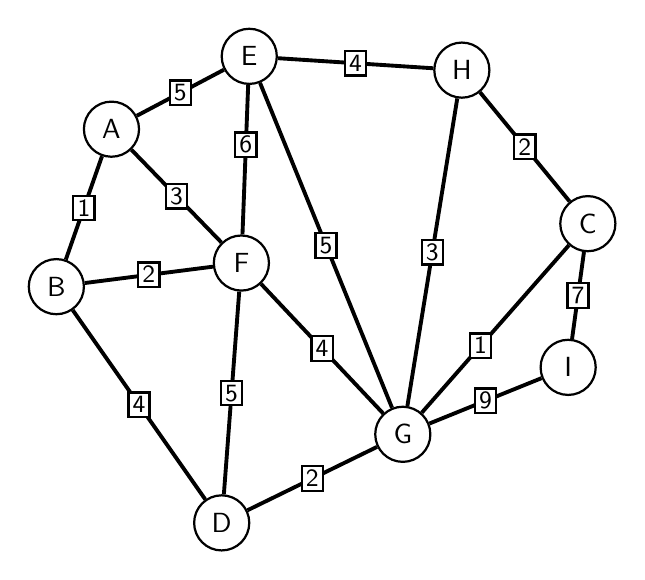
\begin{tikzpicture}[x=2.5cm,y=-2.5cm,
  v/.style={circle,draw,thick,inner sep=0pt,minimum size=7mm,font=\sffamily},
  e/.style={line width=1.4pt},
  w/.style={draw,thick,fill=white,inner sep=1.5pt,font=\sffamily\small}]
\node[v] (A) at (2.20,2.12) {A};
\node[v] (E) at (2.90,1.75) {E};
\node[v] (H) at (3.98,1.82) {H};
\node[v] (C) at (4.62,2.60) {C};
\node[v] (B) at (1.92,2.92) {B};
\node[v] (F) at (2.86,2.80) {F};
\node[v] (I) at (4.52,3.33) {I};
\node[v] (G) at (3.68,3.67) {G};
\node[v] (D) at (2.76,4.12) {D};
\draw[e] (A) -- node[w] {5} (E);
\draw[e] (A) -- node[w] {1} (B);
\draw[e] (A) -- node[w] {3} (F);
\draw[e] (B) -- node[w] {2} (F);
\draw[e] (B) -- node[w] {4} (D);
\draw[e] (E) -- node[w,pos=0.4] {6} (F);
\draw[e] (E) -- node[w] {4} (H);
\draw[e] (E) -- node[w] {5} (G);
\draw[e] (F) -- node[w] {4} (G);
\draw[e] (F) -- node[w] {5} (D);
\draw[e] (H) -- node[w] {3} (G);
\draw[e] (H) -- node[w] {2} (C);
\draw[e] (C) -- node[w,pos=0.6] {1} (G);
\draw[e] (C) -- node[w] {7} (I);
\draw[e] (I) -- node[w] {9} (G);
\draw[e] (D) -- node[w] {2} (G);
\end{tikzpicture}
\end{center}
\end{pastexam}

\begin{pastsoln}
答案：總權重 $23$。 最小生成樹有兩棵：A--B、C--G、B--F、C--H、D--G、E--H、C--I 這 $7$ 條，
再加上 B--D 或 F--G（兩條都是 $4$）其中一條。

\textbf{Kruskal}（資結書第~24.2~節）：$9$ 個頂點、$16$ 條邊，邊依權重由小到大看，兩端已在同一個
集合（會成環）就跳過。 權重相同的邊照字母順序看。
\begin{center}
\small
\begin{tabular}{cllp{0.42\linewidth}}
\toprule
權重 & 邊 & 結果 & 加入後的集合（只列兩個點以上的） \\
\midrule
1 & A--B & 加入 & $\{A, B\}$ \\
1 & C--G & 加入 & $\{A, B\}$, $\{C, G\}$ \\
2 & B--F & 加入 & $\{A, B, F\}$, $\{C, G\}$ \\
2 & C--H & 加入 & $\{A, B, F\}$, $\{C, G, H\}$ \\
2 & D--G & 加入 & $\{A, B, F\}$, $\{C, D, G, H\}$ \\
3 & A--F & 跳過（A--B--F 成環） & \\
3 & G--H & 跳過（G--C--H 成環） & \\
4 & B--D & 加入 & $\{A, B, C, D, F, G, H\}$ \\
4 & E--H & 加入 & $\{A, B, C, D, E, F, G, H\}$ \\
4 & F--G & 跳過（F--B--D--G 成環） & \\
5 & A--E, D--F, E--G & 都跳過 & \\
6 & E--F & 跳過 & \\
7 & C--I & 加入 & 全部 $9$ 個點 \\
\bottomrule
\end{tabular}
\end{center}
加到第 $8$ 條邊（$= 9 - 1$）就停，I--G（$9$）不用看。 總權重
$1 + 1 + 2 + 2 + 2 + 4 + 4 + 7 = 23$。

\begin{center}
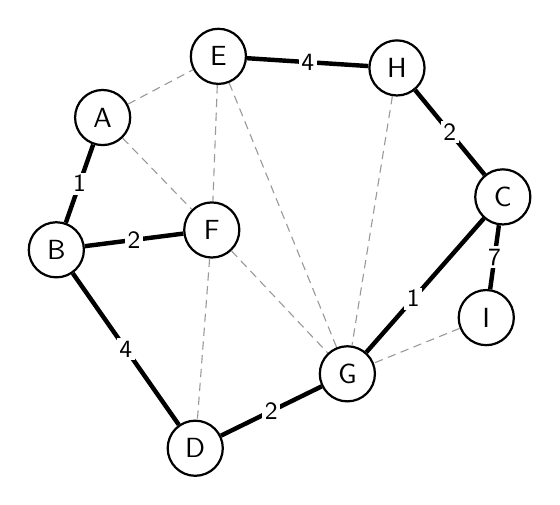
\begin{tikzpicture}[x=2.1cm,y=-2.1cm,
  v/.style={circle,draw,thick,inner sep=0pt,minimum size=7mm,font=\sffamily},
  t/.style={line width=1.6pt},
  n/.style={densely dashed,black!40},
  w/.style={fill=white,inner sep=1pt,font=\sffamily\small}]
\node[v] (A) at (2.20,2.12) {A};
\node[v] (E) at (2.90,1.75) {E};
\node[v] (H) at (3.98,1.82) {H};
\node[v] (C) at (4.62,2.60) {C};
\node[v] (B) at (1.92,2.92) {B};
\node[v] (F) at (2.86,2.80) {F};
\node[v] (I) at (4.52,3.33) {I};
\node[v] (G) at (3.68,3.67) {G};
\node[v] (D) at (2.76,4.12) {D};
\draw[n] (A) -- (E);
\draw[t] (A) -- node[w] {1} (B);
\draw[n] (A) -- (F);
\draw[t] (B) -- node[w] {2} (F);
\draw[t] (B) -- node[w] {4} (D);
\draw[n] (E) -- (F);
\draw[t] (E) -- node[w] {4} (H);
\draw[n] (E) -- (G);
\draw[n] (F) -- (G);
\draw[n] (F) -- (D);
\draw[n] (H) -- (G);
\draw[t] (H) -- node[w] {2} (C);
\draw[t] (C) -- node[w,pos=0.6] {1} (G);
\draw[t] (C) -- node[w] {7} (I);
\draw[n] (I) -- (G);
\draw[t] (D) -- node[w] {2} (G);
\end{tikzpicture}
\end{center}
粗線是最小生成樹的邊，虛線是沒選的邊。

\textbf{為什麼有兩棵。} 第 $4$ 輪如果先看 F--G 再看 B--D，會加入 F--G、跳過 B--D，得到另一棵，
總權重一樣是 $23$。 兩條邊都在環 B--D--G--F--B 上，這個環上另外兩條 D--G（$2$）、B--F（$2$）都
比較輕，B--D 和 F--G 一樣重，是這個環上最重的邊，拿掉哪一條都可以。 資結書定理~24.4 說權重
都不同時最小生成樹唯一；這張圖有相同的權重，所以可能不唯一，但總權重一定相同。

用 Prim（資結書第~24.3~節）從 A 開始也一樣：依序加入 B（A--B 1）、F（B--F 2），這時最輕的跨越邊是
B--D 和 F--G（都是 $4$）。 選 B--D 的話接著是 D（4）、G（D--G 2）、C（C--G 1）、H（C--H 2）、
E（E--H 4）、I（C--I 7），得到上圖那一棵；選 F--G 就得到另一棵。
\end{pastsoln}
